\documentclass[12pt, a4paper]{article}
\usepackage{../../../myconfig} % Gọi file cấu hình chuẩn myconfig.sty

% ==========================================
% BẮT ĐẦU NỘI DUNG TÀI LIỆU - ĐỀ SỐ 2
% ==========================================
\begin{document}

% Tiêu đề đầu đề thi: {Nhãn cam} {Chữ to chính giữa} {Chữ ở góc phải Header}
\titlebox{ĐỀ SỐ 2}{ĐỀ THI GIỮA HỌC KỲ I -- LỚP 12}{Ôn tập GKI}

\textit{\textbf{PHẦN I. Câu trắc nghiệm nhiều phương án lựa chọn. Thí sinh trả lời từ câu 1 đến câu 12. Mỗi câu thí sinh chỉ chọn một phương án.}}

\vspace{0.3cm}

% --- CÂU 1 ---
\questionLinesManual{0}{1}{Cho hàm số $y=f(x)$ có bảng biến thiên như hình bên dưới:
\begin{center}

\begin{tikzpicture}[scale=0.9]
    \tkzTabInit[lgt=1.5,espcl=2.2,deltacl=0.5]{$x$/0.8,$y'$/0.7,$y$/1.8}{$-\infty$,$0$,$1$,$+\infty$}
    \tkzTabLine{,-,d,-,0,+,}
    \tkzTabVar{+/$+\infty$, -D+/$-\infty$/$+\infty$, -/$-2$, +/$+\infty$}
\end{tikzpicture}
\end{center}
Khẳng định nào sau đây là sai?}{%
    \begin{tasks}(2)
        \task Hàm số đồng biến trên khoảng $(2;+\infty)$.
        \task Hàm số nghịch biến trên khoảng $(-\infty;-1)$.
        \task Hàm số đồng biến trên khoảng $(-2;+\infty)$.
        \task Hàm số nghịch biến trên khoảng $(0;1)$.
    \end{tasks}
}

% --- CÂU 2 ---
\questionLinesManual{0}{2}{Tìm số đường tiệm cận của đồ thị hàm số $y=\dfrac{2x-1}{x^2+1}$.}{%
    \begin{tasks}(4)
        \task $3$.
        \task $2$.
        \task $0$.
        \task $1$.
    \end{tasks}
}

% --- CÂU 3 ---
\questionLinesManual{0}{3}{Cho hàm số $y=f(x)$ xác định, liên tục trên tập $\mathbb{R}$ và có đồ thị là đường cong trong hình vẽ bên. Hàm số $f(x)$ đạt cực đại tại điểm nào dưới đây?
\begin{center}
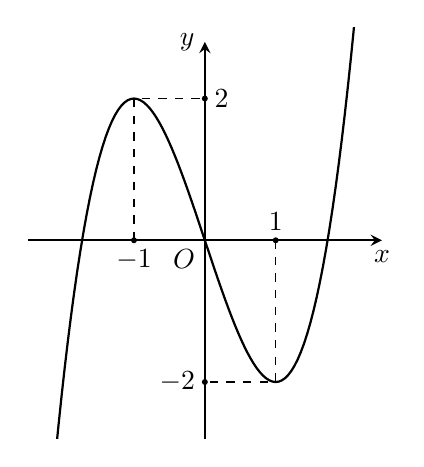
\begin{tikzpicture}[scale=0.9, >=stealth]
    \clip (-2.5,-2.8) rectangle (2.7,3);
    \draw[->, thick] (-2.5,0) -- (2.5,0) node[below] {$x$};
    \draw[->, thick] (0,-2.8) -- (0,2.8) node[left] {$y$};
    \node[below left] at (0,0) {$O$};
    
    \draw[thick, domain=-2.2:2.2, samples=100] plot (\x, {(\x)^3 - 3*(\x)});
    
    \draw[dashed] (-1,0) -- (-1,2) -- (0,2);
    \draw[dashed] (1,0) -- (1,-2) -- (0,-2);
    
    \fill (-1,0) circle (1.2pt) node[below] {$-1$};
    \fill (1,0) circle (1.2pt) node[above] {$1$};
    \fill (0,2) circle (1.2pt) node[right] {$2$};
    \fill (0,-2) circle (1.2pt) node[left] {$-2$};
\end{tikzpicture}
\end{center}
}{%
    \begin{tasks}(4)
        \task $x=-2$.
        \task $x=1$.
        \task $x=-1$.
        \task $x=2$.
    \end{tasks}
}

% --- CÂU 4 ---
\questionLinesManual{0}{4}{Trong hệ trục toạ độ $Oxyz$, cho tam giác $ABC$ có $A(1;0;2)$, $B(3;-2;4)$ và $C(2;-1;3)$. Toạ độ trọng tâm $G$ của $\triangle ABC$ là}{%
    \begin{tasks}(4)
        \task $G(2;-1;3)$.
        \task $G(4;-2;6)$.
        \task $G(2;1;3)$.
        \task $G(6;-3;9)$.
    \end{tasks}
}

% --- CÂU 5 ---
\questionLinesManual{0}{5}{Đường cong trong hình bên là đồ thị của hàm số nào dưới đây?
\begin{center}
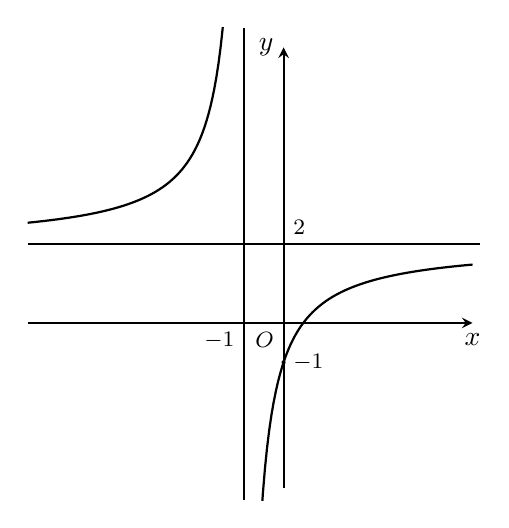
\begin{tikzpicture}[scale=0.5, >=stealth]
    % Giới hạn vùng vẽ đủ cao để lấy trọn nhánh cong phía trên
    \clip (-6.5, -4.5) rectangle (5.0, 7.5);

    % Trục tọa độ Ox, Oy được mở rộng
    \draw[->, line width=0.7pt] (-6.5, 0) -- (4.8, 0) node[below] {$x$};
    \draw[->, line width=0.7pt] (0, -4.2) -- (0, 7.0) node[left] {$y$};
    \node[below left, font=\footnotesize] at (0, 0) {$O$};

    % Tiệm cận đứng: x = -1
    \draw[line width=0.6pt] (-1, -4.5) -- (-1, 7.5);
    % Tiệm cận ngang: y = 2
    \draw[line width=0.6pt] (-6.5, 2) -- (5.0, 2);

    % Nhãn các giá trị trên trục
    \node[below left, font=\footnotesize] at (-1, 0) {$-1$};
    \node[above right, font=\footnotesize] at (0, 2) {$2$};

    % Đồ thị hàm số y = (2x - 1)/(x + 1)
    % Nhánh trên bên trái (x < -1) thể hiện rõ đường cong tiệm cận
    \draw[thick, domain=-6.5:-1.45, samples=100] plot (\x, {(2*(\x)-1)/((\x)+1)});
    % Nhánh dưới bên phải (x > -1)
    \draw[thick, domain=-0.58:4.8, samples=100] plot (\x, {(2*(\x)-1)/((\x)+1)});

    % Giao điểm với trục Oy: (0, -1)
    \fill (0, -1) circle (1.5pt);
    \node[right, font=\footnotesize] at (0, -1) {$-1$};
\end{tikzpicture}
\end{center}
}{%
    \begin{tasks}(2)
        \task $y=\dfrac{2x+1}{x-1}$.
        \task $y=\dfrac{2x+1}{x+1}$.
        \task $y=\dfrac{2x-1}{x+1}$.
        \task $y=\dfrac{x-2}{x+1}$.
    \end{tasks}
}

% --- CÂU 6 ---
\questionLinesManual{0}{6}{Tìm giá trị nhỏ nhất của hàm số $y=x^3-3x+4$ trên đoạn $[0;2]$.}{%
    \begin{tasks}(4)
        \task $\min\limits_{[0;2]} y = 1$.
        \task $\min\limits_{[0;2]} y = 2$.
        \task $\min\limits_{[0;2]} y = 4$.
        \task $\min\limits_{[0;2]} y = 0$.
    \end{tasks}
}

% --- CÂU 7 ---
\questionLinesManual{0}{7}{Đồ thị hàm số $y=\dfrac{x^2-x-1}{x-2}$ có dạng:

}{%
    \begin{tasks}(2)
        \task {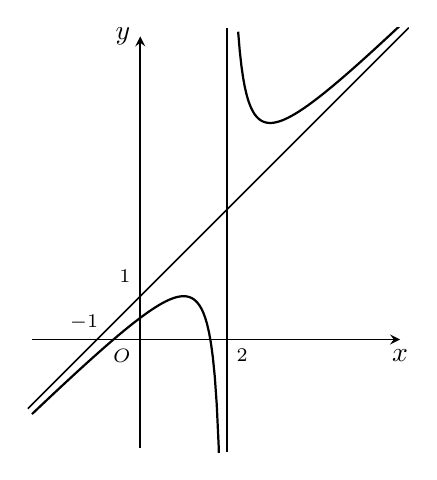
\begin{tikzpicture}[scale=0.55, >=stealth]
    % Khóa khung nhìn
    \clip (-2.6, -2.6) rectangle (6.2, 7.2);

    % Trục tọa độ Ox, Oy
    \draw[->, line width=0.6pt] (-2.5, 0) -- (6.0, 0) node[below] {$x$};
    \draw[->, line width=0.6pt] (0, -2.5) -- (0, 7.0) node[left] {$y$};
    \node[below left, font=\scriptsize] at (0, 0) {$O$};

    % Tiệm cận đứng: x = 2
    \draw[line width=0.6pt] (2, -2.6) -- (2, 7.2);
    % Tiệm cận xiên: y = x + 1
    \draw[line width=0.6pt] (-2.6, -1.6) -- (6.2, 7.2);

    % Nhãn tọa độ
    \node[above, font=\scriptsize] at (-1.3, 0) {$-1$};
    \node[above left, font=\scriptsize] at (0, 1.1) {$1$};
    \node[below right, font=\scriptsize] at (2, 0) {$2$};

    % Đồ thị hàm số y = (x^2 - x - 1)/(x - 2)
    % Nhánh trái (x < 2)
    \draw[thick, domain=-2.5:1.9, samples=100] plot (\x, {((\x)^2 - (\x) - 1)/((\x) - 2)});
    % Nhánh phải (x > 2)
    \draw[thick, domain=2.26:6.0, samples=100] plot (\x, {((\x)^2 - (\x) - 1)/((\x) - 2)});
\end{tikzpicture}}
        \task 
        {% ==================== HÌNH B ====================
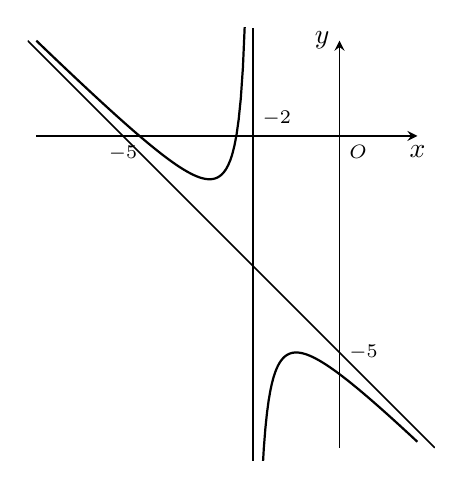
\begin{tikzpicture}[scale=0.55, >=stealth]
    % Khóa khung nhìn
    \clip (-7.2, -7.5) rectangle (2.2, 2.5);

    % Trục tọa độ Ox, Oy
    \draw[->, line width=0.6pt] (-7.0, 0) -- (1.8, 0) node[below] {$x$};
    \draw[->, line width=0.6pt] (0, -7.2) -- (0, 2.2) node[left] {$y$};
    \node[below right, font=\scriptsize] at (0, 0) {$O$};

    % Tiệm cận đứng: x = -2
    \draw[line width=0.6pt] (-2, -7.5) -- (-2, 2.5);
    % Tiệm cận xiên: y = -x - 5
    \draw[line width=0.6pt] (-7.2, 2.2) -- (2.2, -7.2);

    % Nhãn các số trên trục
    \node[below, font=\scriptsize] at (-5, 0) {$-5$};
    \node[above right, font=\scriptsize] at (-2, 0) {$-2$};
    \node[right, font=\scriptsize] at (0, -5) {$-5$};

    % Đồ thị: y = -x - 5 - 1/(x + 2)
    % Nhánh trái (x < -2) uốn cong có cực tiểu
    \draw[thick, domain=-7.0:-2.18, samples=100] plot (\x, {-(\x) - 5 - 1/((\x) + 2)});
    % Nhánh phải (x > -2) uốn cong có cực đại
    \draw[thick, domain=-1.82:1.8, samples=100] plot (\x, {-(\x) - 5 - 1/((\x) + 2)});
\end{tikzpicture}}
        \task 
        {% ==================== HÌNH C ====================
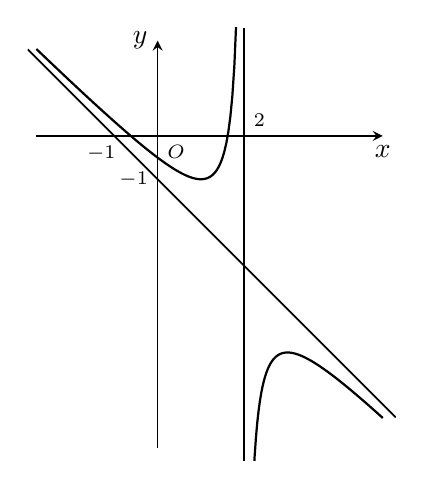
\begin{tikzpicture}[scale=0.55, >=stealth]
    % Khóa khung nhìn
    \clip (-3.0, -7.5) rectangle (5.5, 2.5);

    % Trục tọa độ Ox, Oy
    \draw[->, line width=0.6pt] (-2.8, 0) -- (5.2, 0) node[below] {$x$};
    \draw[->, line width=0.6pt] (0, -7.2) -- (0, 2.2) node[left] {$y$};
    \node[below right, font=\scriptsize] at (0, 0) {$O$};

    % Tiệm cận đứng: x = 2
    \draw[line width=0.6pt] (2, -7.5) -- (2, 2.5);
    % Tiệm cận xiên: y = -x - 1
    \draw[line width=0.6pt] (-3.0, 2.0) -- (5.5, -6.5);

    % Nhãn các số trên trục
    \node[below, font=\scriptsize] at (-1.3, 0) {$-1$};
    \node[left, font=\scriptsize] at (0, -1) {$-1$};
    \node[above right, font=\scriptsize] at (2, 0) {$2$};

    % Đồ thị: y = -x - 1 - 1/(x - 2)
    % Nhánh trái (x < 2) uốn cong có cực tiểu
    \draw[thick, domain=-2.8:1.82, samples=100] plot (\x, {-(\x) - 1 - 1/((\x) - 2)});
    % Nhánh phải (x > 2) uốn cong có cực đại
    \draw[thick, domain=2.18:5.2, samples=100] plot (\x, {-(\x) - 1 - 1/((\x) - 2)});
\end{tikzpicture}}
        \task 
        {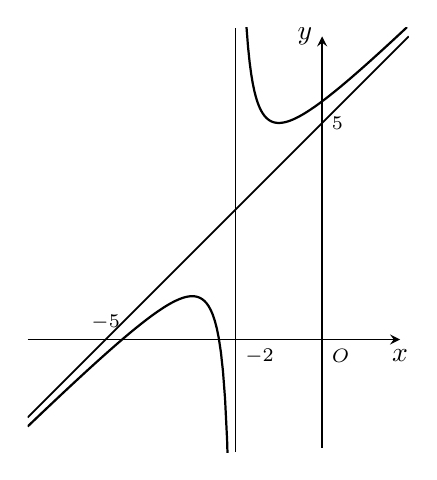
\begin{tikzpicture}[scale=0.55, >=stealth]
    % Khóa khung nhìn
    \clip (-6.8, -2.6) rectangle (2.0, 7.2);

    % Trục tọa độ Ox, Oy
    \draw[->, line width=0.6pt] (-6.8, 0) -- (1.8, 0) node[below] {$x$};
    \draw[->, line width=0.6pt] (0, -2.5) -- (0, 7.0) node[left] {$y$};
    \node[below right, font=\scriptsize] at (0, 0) {$O$};

    % Tiệm cận đứng: x = -2
    \draw[line width=0.6pt] (-2, -2.6) -- (-2, 7.2);
    % Tiệm cận xiên: y = x + 5
    \draw[line width=0.6pt] (-6.8, -1.8) -- (2.0, 7.0);

    % Nhãn tọa độ
    \node[above, font=\scriptsize] at (-5, 0) {$-5$};
    \node[below right, font=\scriptsize] at (-2, 0) {$-2$};
    \node[right, font=\scriptsize] at (0, 5) {$5$};

    % Đồ thị minh họa: y = x + 5 + 1/(x + 2)
    \draw[thick, domain=-6.8:-2.1, samples=100] plot (\x, {(\x) + 5 + 1/((\x) + 2)});
    \draw[thick, domain=-1.75:1.96, samples=100] plot (\x, {(\x) + 5 + 1/((\x) + 2)});
\end{tikzpicture}}
    \end{tasks}
}

% --- CÂU 8 ---
\questionLinesManual{0}{8}{Cho hình lập phương $ABCD.A'B'C'D'$. Số vectơ khác vectơ $\vec{0}$ lập từ các đỉnh của hình lập phương bằng $\vec{AB}$ là}{%
    \begin{tasks}(4)
        \task $2$.
        \task $5$.
        \task $4$.
        \task $3$.
    \end{tasks}
}

% --- CÂU 9 ---
\questionLinesManual{0}{9}{Gọi $M, N$ lần lượt là giá trị cực đại, giá trị cực tiểu của hàm số $y=\dfrac{x^2+3x+3}{x+2}$. Khi đó giá trị của biểu thức $M^2 - N$ bằng}{%
    \begin{tasks}(4)
        \task $6$.
        \task $7$.
        \task $9$.
        \task $8$.
    \end{tasks}
}

% --- CÂU 10 ---
\questionLinesManual{0}{10}{Một loại vi khuẩn được tiêm một loại thuốc kích thích sự sinh sản. Sau $t$ phút, số vi khuẩn được xác định theo công thức $N(t)=1000+30t^2-t^3$, trong đó $0 \le t \le 30$. Hỏi sau bao nhiêu phút thì số vi khuẩn đạt số lượng nhiều nhất?}{%
    \begin{tasks}(4)
        \task $1100$.
        \task $20$.
        \task $1200$.
        \task $10$.
    \end{tasks}
}

% --- CÂU 11 ---
\questionLinesManual{0}{11}{Trong không gian với hệ toạ độ $Oxyz$, cho ba điểm $M(1;1;1)$, $N(2;3;4)$, $P(7;7;5)$. Để tứ giác $MNPQ$ là hình bình hành thì toạ độ điểm $Q$ là}{%
    \begin{tasks}(4)
        \task $Q(6;5;2)$.
        \task $Q(-6;5;2)$.
        \task $Q(6;-5;2)$.
        \task $Q(-6;-5;-2)$.
    \end{tasks}
}

% --- CÂU 12 ---
\questionLinesManual{0}{12}{Cho tứ diện $ABCD$ có $M, N$ lần lượt là trung điểm cạnh $AB$ và $CD$. Đặt $\vec{AB}=\vec{b}$, $\vec{AC}=\vec{c}$, $\vec{AD}=\vec{d}$. Khẳng định nào sau đây đúng?}{%
    \begin{tasks}(2)
        \task $\vec{MN} = \dfrac{1}{2}(\vec{b}+\vec{c}-\vec{d})$.
        \task $\vec{MN} = \dfrac{1}{2}(\vec{c}+\vec{d}-\vec{b})$.
        \task $\vec{MN} = \dfrac{1}{2}(\vec{b}+\vec{d}-\vec{c})$.
        \task $\vec{MN} = \dfrac{1}{2}(\vec{b}+\vec{c}+\vec{d})$.
    \end{tasks}
}


\textit{\textbf{PHẦN II. Câu trắc nghiệm đúng sai. Thí sinh trả lời từ Câu 13 đến Câu 16. Trong mỗi ý a), b), c), d) ở mỗi câu, thí sinh chọn đúng hoặc sai.}}

\vspace{0.3cm}

% --- CÂU 13 (Tương ứng Câu 1 Phần II) ---
\questionTrueFalse{0}{13}{Cho hàm số $y=f(x)$ liên tục trên tập $\mathbb{R}$ và có bảng biến thiên như sau:
\begin{center}

\begin{tikzpicture}[scale=0.95]
    \tkzTabInit[lgt=1.2,espcl=2.2,deltacl=0.5]{$x$/0.8,$y'$/0.7,$y$/1.8}{$-\infty$,$-1$,$2$,$+\infty$}
    \tkzTabLine{,+,0,-,0,+,}
    \tkzTabVar{-/$-\infty$, +/$5$, -/$-2$, +/$+\infty$}
\end{tikzpicture}
\end{center}
Xét tính đúng -- sai của các mệnh đề sau:}{
    \textbf{a)} & Hàm số đồng biến trên khoảng $(0;2)$.
    & \textcolor{amberorange}{$\bigcirc$} & \textcolor{amberorange}{$\bigcirc$} \\ \hline
    
    \textbf{b)} & $\max\limits_{[-\infty;2]} f(x) = 5$.
    & \textcolor{amberorange}{$\bigcirc$} & \textcolor{amberorange}{$\bigcirc$} \\ \hline
    
    \textbf{c)} & Hàm số có 3 cực trị.
    & \textcolor{amberorange}{$\bigcirc$} & \textcolor{amberorange}{$\bigcirc$} \\ \hline
    
    \textbf{d)} & Phương trình $f(x)=0$ có 3 nghiệm phân biệt.
    & \textcolor{amberorange}{$\bigcirc$} & \textcolor{amberorange}{$\bigcirc$} \\
}

% --- CÂU 14 (Tương ứng Câu 2 Phần II) ---
\questionTrueFalse{0}{14}{Cho hàm số $y=f(x)$ có đồ thị như hình vẽ sau:
\begin{center}
\begin{tikzpicture}[scale=0.85, >=stealth]
    % Khóa khung nhìn để đồ thị không bị tràn
    \clip (-4.5, -4.5) rectangle (4.5, 4.2);

    % Trục tọa độ Ox, Oy
    \draw[->, line width=0.7pt] (-4.2, 0) -- (4.2, 0) node[below] {$x$};
    \draw[->, line width=0.7pt] (0, -4.2) -- (0, 3.8) node[left] {$y$};
    \node[below left, font=\footnotesize] at (0, 0) {$O$};

    % Tiệm cận đứng: x = -1
    \draw[line width=0.6pt] (-1, -4.5) -- (-1, 4.2);
    \node[above left, font=\footnotesize] at (-1, 0) {$-1$};

    % Tiệm cận xiên: y = -0.5*x - 0.5 (cắt Ox tại -1, Oy tại -0.5)
    \draw[line width=0.6pt] (-4.5, 1.75) -- (4.5, -2.75);

    % Các đường dóng nét đứt tới điểm cực tiểu (-2; 1.5)
    \draw[dashed, line width=0.5pt] (-2, 0) -- (-2, 1.5) -- (0, 1.5);
    \fill (-2, 0) circle (1.2pt) node[below, font=\footnotesize] {$-2$};
    \fill (0, 1.5) circle (1.2pt) node[right, font=\footnotesize] {$\dfrac{3}{2}$};

    % Điểm mốc trên trục và điểm cực đại (0; -0.5)
    \fill (0, -0.5) circle (1.2pt);
    \node[right, font=\footnotesize] at (0.05, -0.6) {$-0.5$};
   

    % Nhánh trái (x < -1): có điểm cực tiểu tại (-2; 1.5)
    \draw[thick, domain=-4.2:-1.22, samples=100] 
        plot (\x, {-0.5*(\x) - 0.5 - 1/((\x) + 1)});

    % Nhánh phải (x > -1): có điểm cực đại tại (0; -0.5)
    \draw[thick, domain=-0.78:4.2, samples=100] 
        plot (\x, {-0.5*(\x) - 0.5 - 1/((\x) + 1)});
\end{tikzpicture}
\end{center}
Xét tính đúng -- sai của các mệnh đề sau:}{
    \textbf{a)} & Hàm số đồng biến trên khoảng $(-\infty;-1)$.
    & \textcolor{amberorange}{$\bigcirc$} & \textcolor{amberorange}{$\bigcirc$} \\ \hline
    
    \textbf{b)} & Hàm số đạt cực đại tại $x=-2$.
    & \textcolor{amberorange}{$\bigcirc$} & \textcolor{amberorange}{$\bigcirc$} \\ \hline
    
    \textbf{c)} & Giá trị nhỏ nhất của hàm số trên $(-\infty;-1)$ là $\dfrac{3}{2}$.
    & \textcolor{amberorange}{$\bigcirc$} & \textcolor{amberorange}{$\bigcirc$} \\ \hline
    
    \textbf{d)} & Tiệm cận đứng của đồ thị hàm số là $x=-1$.
    & \textcolor{amberorange}{$\bigcirc$} & \textcolor{amberorange}{$\bigcirc$} \\
}

% --- CÂU 15 (Tương ứng Câu 3 Phần II) ---
\questionTrueFalse{0}{15}{Hàm số $y=\dfrac{ax+2}{cx+b}$ có đồ thị như hình vẽ:
\begin{center}
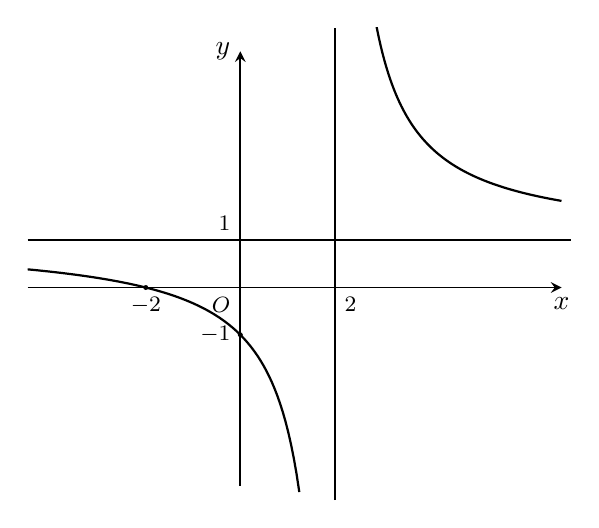
\begin{tikzpicture}[scale=0.6, >=stealth]
    % Khóa khung nhìn để hai nhánh đồ thị không bị phóng vọt ra ngoài
    \clip (-4.5, -4.5) rectangle (7.0, 5.5);

    % Trục tọa độ Ox, Oy
    \draw[->, line width=0.7pt] (-4.5, 0) -- (6.8, 0) node[below] {$x$};
    \draw[->, line width=0.7pt] (0, -4.2) -- (0, 5.0) node[left] {$y$};
    \node[below left, font=\footnotesize] at (0, 0) {$O$};

    % Đường tiệm cận đứng x = 2 và tiệm cận ngang y = 1
    \draw[line width=0.6pt] (2, -4.5) -- (2, 5.5);
    \draw[line width=0.6pt] (-4.5, 1) -- (7.0, 1);

    % Nhãn các giá trị trên trục
    \node[above left, font=\footnotesize] at (0, 1) {$1$};
    \node[below right, font=\footnotesize] at (2, 0) {$2$};

    % Điểm cắt trục Ox (-2; 0) và Oy (0; -1)
    \fill (-2, 0) circle (1.5pt);
    \node[below, font=\footnotesize] at (-2, 0) {$-2$};
    
    \fill (0, -1) circle (1.5pt);
    \node[left, font=\footnotesize] at (0, -1) {$-1$};

    % Đồ thị hàm số y = (x + 2)/(x - 2)
    % Nhánh trái (x < 2): đi qua (-2; 0) và (0; -1)
    \draw[thick, domain=-4.5:1.25, samples=100] plot (\x, {((\x) + 2)/((\x) - 2)});
    
    % Nhánh phải (x > 2): tiệm cận x = 2 và y = 1
    \draw[thick, domain=2.85:6.8, samples=100] plot (\x, {((\x) + 2)/((\x) - 2)});
\end{tikzpicture}
\end{center}
Xét tính đúng -- sai của các mệnh đề sau:}{
    \textbf{a)} & Các hệ số $a, b$ thoả mãn $a \cdot b > 0$.
    & \textcolor{amberorange}{$\bigcirc$} & \textcolor{amberorange}{$\bigcirc$} \\ \hline
    
    \textbf{b)} & Các hệ số $a, c$ thoả mãn $a \cdot c > 0$.
    & \textcolor{amberorange}{$\bigcirc$} & \textcolor{amberorange}{$\bigcirc$} \\ \hline
    
    \textbf{c)} & Các hệ số $b, c$ thoả mãn $b \cdot c > 0$.
    & \textcolor{amberorange}{$\bigcirc$} & \textcolor{amberorange}{$\bigcirc$} \\ \hline
    
    \textbf{d)} & Các hệ số $a, b, c$ thoả mãn $a+b+c=0$.
    & \textcolor{amberorange}{$\bigcirc$} & \textcolor{amberorange}{$\bigcirc$} \\
}

% --- CÂU 16 (Tương ứng Câu 4 Phần II) ---
\questionTrueFalse{0}{16}{Trong không gian với hệ toạ độ $Oxyz$, cho ba điểm $A(3;-1;1)$, $B(4;-2;0)$ và $C(3;-2;-2)$. Xét tính đúng -- sai của các mệnh đề sau:}{
    \textbf{a)} & $\vec{AB} \cdot \vec{AC} = 4$.
    & \textcolor{amberorange}{$\bigcirc$} & \textcolor{amberorange}{$\bigcirc$} \\ \hline
    
    \textbf{b)} & Hình chiếu của điểm $A$ trên mặt phẳng toạ độ $(Oxy)$ là $A'(3;-1;0)$.
    & \textcolor{amberorange}{$\bigcirc$} & \textcolor{amberorange}{$\bigcirc$} \\ \hline
    
    \textbf{c)} & Nếu $(\vec{AB}, \vec{AC}) = \alpha$ thì $\cos\alpha = \dfrac{\sqrt{30}}{15}$.
    & \textcolor{amberorange}{$\bigcirc$} & \textcolor{amberorange}{$\bigcirc$} \\ \hline
    
    \textbf{d)} & Nếu đường thẳng $AB$ cắt mặt phẳng toạ độ $(Oxz)$ tại $M$ thì $M(2;0;2)$.
    & \textcolor{amberorange}{$\bigcirc$} & \textcolor{amberorange}{$\bigcirc$} \\
}



\textit{\textbf{PHẦN III. Câu trắc nghiệm trả lời ngắn. Thí sinh trả lời từ Câu 17 đến Câu 22.}}

\vspace{0.3cm}

% --- CÂU 17 (Tương ứng Câu 1 Phần III) ---
\questionShortAnswer{0}{17}{Cho hàm số $y=f(x)=\dfrac{1}{3}x^3-x^2-3x+\dfrac{1}{3}$. Tìm giá trị cực tiểu của hàm số (kết quả làm tròn đến hàng phần chục).
}

% --- CÂU 18 (Tương ứng Câu 2 Phần III) ---
\questionShortAnswer{0}{18}{Cho hàm số $y=f(x)$ có bảng biến thiên như sau:
\begin{center}

\begin{tikzpicture}[scale=0.95]
    \tkzTabInit[lgt=1.2,espcl=2.2,deltacl=0.5]{$x$/0.8,$y'$/0.7,$y$/1.8}{$-\infty$,$-1$,$1$,$+\infty$}
    \tkzTabLine{,+,0,-,0,+,}
    \tkzTabVar{-/$1$, +/$3$, -/$\dfrac{1}{3}$, +/$1$}
\end{tikzpicture}
\end{center}
Tìm số nghiệm của phương trình $2f^2(x)-3f(x)+1=0$.
}

% --- CÂU 19 (Tương ứng Câu 3 Phần III) ---
\questionShortAnswer{0}{19}{Đợt xuất khẩu gạo của tỉnh A thường kéo dài trong 2 tháng (60 ngày). Người ta nhận thấy số lượng xuất khẩu gạo tính theo ngày thứ $t$ được xác định bởi công thức:
\[ S(t) = \dfrac{2}{5}t^3 - 63t^2 + 3240t - 3100 \quad (\text{tấn}) \quad \text{với } (1 \le t \le 60). \]
Hỏi trong 60 ngày đó thì ngày thứ mấy có số lượng xuất khẩu gạo cao nhất?
}

% --- CÂU 20 (Tương ứng Câu 4 Phần III) ---
\questionShortAnswer{0}{20}{Một xe buýt có sức chứa tối đa là 50 hành khách. Nếu một chuyến xe buýt chở $x$ hành khách thì giá tiền cho mỗi hành khách là $20\left(3 - \dfrac{x}{40}\right)^2$ (nghìn đồng). Tính số tiền (nghìn đồng) thu được nhiều nhất của một chuyến xe buýt.
}

% --- CÂU 21 (Tương ứng Câu 5 Phần III) ---
\questionShortAnswer{0}{21}{Giả sử chi phí tiền xăng $C$ (đồng) phụ thuộc tốc độ trung bình $v$ (km/h) theo công thức:
\[ C(v) = \dfrac{16000}{v} + \dfrac{5}{2}v \quad (0 < v \le 120). \]
Tính tốc độ trung bình để chi phí tiền xăng là ít nhất.
}

% --- CÂU 22 (Tương ứng Câu 6 Phần III) ---
\questionShortAnswer{0}{22}{Hình minh hoạ sơ đồ một ngôi nhà trong hệ trục toạ độ $Oxyz$, trong đó nền nhà, bốn bức tường và hai mái nhà đều là hình chữ nhật. Gọi $\widehat{PFE}=\alpha$ là góc dốc của mái nhà. Tính $\cos\alpha$ (làm tròn kết quả đến phần trăm).
\begin{center}
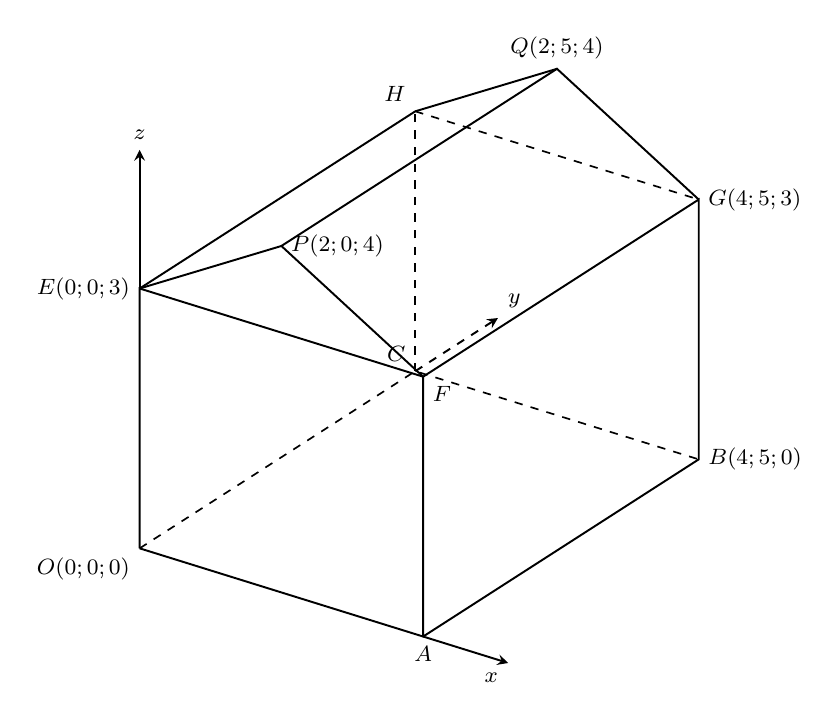
\begin{tikzpicture}[
    x={(0.9cm, -0.28cm)},   % vector chỉ phương trục Ox
    y={(0.7cm, 0.45cm)},    % vector chỉ phương trục Oy (xiên chéo vào trong)
    z={(0cm, 1.1cm)},       % vector chỉ phương trục Oz (thẳng đứng)
    >=stealth
]
    % --- ĐỊNH NGHĨA TỌA ĐỘ CHUẨN CỦA TỪNG ĐIỂM ---
    \coordinate (O) at (0, 0, 0);
    \coordinate (A) at (4, 0, 0);
    \coordinate (B) at (4, 5, 0);
    \coordinate (C) at (0, 5, 0);

    \coordinate (E) at (0, 0, 3);
    \coordinate (F) at (4, 0, 3);
    \coordinate (G) at (4, 5, 3);
    \coordinate (H) at (0, 5, 3);

    \coordinate (P) at (2, 0, 4);
    \coordinate (Q) at (2, 5, 4);

    % --- NÉT KHUẤT (NÉT ĐỨT) ---
    \draw[dashed, line width=0.6pt] (O) -- (C) -- (B);
    \draw[dashed, line width=0.6pt] (C) -- (H);
    \draw[dashed, line width=0.6pt]  (H) -- (G);

    % Trục Oy nét đứt kéo dài ra sau
    \draw[->, dashed, line width=0.7pt] (C) -- (0, 6.5, 0) node[above right, font=\footnotesize] {$y$};

    % --- NÉT THẤY (NÉT LIỀN) ---
    % Nền và cột tường
    \draw[line width=0.7pt] (O) -- (A) -- (B) -- (G) -- (F) -- (A);
    \draw[line width=0.7pt] (O) -- (E) -- (F);
    \draw[line width=0.7pt] (E) -- (H) -- (Q);
    % Mái nhà phía trước (tam giác EPF)
    \draw[line width=0.7pt] (E) -- (P) -- (F);
    % Mái nhà phía sau và nóc nhà
    \draw[line width=0.7pt] (P) -- (Q) -- (G);

    % --- CÁC TRỤC TỌA ĐỘ Ox, Oz ---
    \draw[->, line width=0.7pt] (A) -- (5.2, 0, 0) node[below left, font=\footnotesize] {$x$};
    \draw[->, line width=0.7pt] (E) -- (0, 0, 4.6) node[above, font=\footnotesize] {$z$};

    % --- TÊN VÀ TỌA ĐỘ CÁC ĐIỂM ---
    \node[below left, font=\footnotesize] at (O) {$O(0;0;0)$};
    \node[below, font=\footnotesize] at (A) {$A$};
    \node[right, font=\footnotesize] at (B) {$B(4;5;0)$};
    \node[above left, font=\footnotesize] at (C) {$C$};

    \node[left, font=\footnotesize] at (E) {$E(0;0;3)$};
    \node[below right, font=\footnotesize] at (F) {$F$};
    \node[right, font=\footnotesize] at (G) {$G(4;5;3)$};
    \node[above left, font=\footnotesize] at (H) {$H$};

    \node[right, font=\footnotesize] at (P) {$P(2;0;4)$};
    \node[above, font=\footnotesize] at (Q) {$Q(2;5;4)$};
\end{tikzpicture}
\end{center}
}

\end{document}

% =========================================================================
% BẢNG ĐÁP ÁN THAM KHẢO CHO ĐỀ SỐ 2:
% =========================================================================
% PHẦN I:
% 1.C | 2.D | 3.C | 4.A | 5.C | 6.B | 7.A | 8.D | 9.D | 10.B | 11.A | 12.B
%
% PHẦN II:
% Câu 13 (Câu 1): a) Sai | b) Đúng | c) Sai  | d) Đúng
% Câu 14 (Câu 2): a) Sai | b) Sai  | c) Đúng | d) Đúng
% Câu 15 (Câu 3): a) Sai | b) Đúng | c) Sai  | d) Đúng
% Câu 16 (Câu 4): a) Đúng | b) Đúng | c) Sai | d) Đúng
%
% PHẦN III:
% Câu 17 (Câu 1): -8,7
% Câu 18 (Câu 2): 3
% Câu 19 (Câu 3): 45
% Câu 20 (Câu 4): 3200
% Câu 21 (Câu 5): 80
% Câu 22 (Câu 6): 0,89